\pdfminorversion=7
\documentclass[10pt,twocolumn]{article}
\usepackage[letterpaper,top=0.49in,bottom=0.52in,left=0.55in,right=0.55in,columnsep=0.20in]{geometry}
\usepackage[T1]{fontenc}
\usepackage{lmodern}
\usepackage{microtype}
\usepackage{graphicx}
\usepackage{booktabs}
\usepackage{float}
\usepackage{amsmath}
\usepackage{url}
\usepackage[hidelinks]{hyperref}
\usepackage{xcolor}
\hypersetup{
  pdftitle={C-GEAR: Calibrated Genetic Efficiency-Aware Rank Allocation for Incremental LoRA Fine-Tuning},
  pdfauthor={Ali Naghiloo and Mohammad Farid Barenji},
  pdfsubject={Deep Learning final project, Sharif University of Technology}
}

\setlength{\parindent}{0.9em}
\setlength{\parskip}{0pt}
\setlength{\textfloatsep}{5pt plus 1pt minus 1pt}
\setlength{\dbltextfloatsep}{5pt plus 1pt minus 1pt}
\setlength{\floatsep}{4pt plus 1pt minus 1pt}
\setlength{\intextsep}{4pt plus 1pt minus 1pt}
\setlength{\abovecaptionskip}{2pt}
\setlength{\belowcaptionskip}{0pt}
\renewcommand{\topfraction}{0.95}
\renewcommand{\dbltopfraction}{0.95}
\renewcommand{\textfraction}{0.04}
\renewcommand{\dblfloatpagefraction}{0.85}
\makeatletter
\renewcommand\section{\@startsection{section}{1}{\z@}{4pt plus 1pt minus 1pt}{2pt}{\normalfont\bfseries\small}}
\renewcommand\subsection{\@startsection{subsection}{2}{\z@}{3pt plus 1pt minus 1pt}{1pt}{\normalfont\bfseries\footnotesize}}
\makeatother
\makeatletter
\long\def\@makecaption#1#2{\vskip\abovecaptionskip\sbox\@tempboxa{\footnotesize\textbf{#1.} #2}\ifdim \wd\@tempboxa >\hsize \footnotesize\textbf{#1.} #2\par \else \global \@minipagefalse \hb@xt@\hsize{\hfil\box\@tempboxa\hfil}\fi\vskip\belowcaptionskip}
\makeatother

% Generated by regenerate_six_seed_analysis.py; do not edit by hand.
\newcommand{\GreedyAccuracy}{87.30}
\newcommand{\CgearAccuracy}{88.09}
\newcommand{\AccuracyGain}{0.78}
\newcommand{\SelectedPairedReduction}{3.55}
\newcommand{\FinalPairedReduction}{13.86}
\newcommand{\CgearWins}{4}
\newcommand{\CgearTies}{0}
\newcommand{\CgearLosses}{2}


\title{\vspace{-1.2em}\textbf{C-GEAR: Calibrated Genetic Efficiency-Aware Rank Allocation\\for Incremental LoRA Fine-Tuning}\vspace{-0.45em}}
\author{\small Ali Naghiloo (404200139) \quad Mohammad Farid Barenji (404203169)\\[-1pt]
\footnotesize Sharif University of Technology, Department of Electrical Engineering\\[-1pt]
\footnotesize Deep Learning --- Instructor: Dr. Bejani; Mentor: Eng. Mehran Advand}
\date{\vspace{-1.1em}}

\begin{document}
\maketitle
\vspace{-1.35em}

\begin{abstract}
Incremental LoRA avoids fixing a large adapter rank in advance, but IncreLoRA assigns each new component through a local importance-based Greedy rule and continues growing toward a preset target. We introduce \emph{C-GEAR}, which anchors evolutionary candidate generation at that rule, calibrates candidate updates on training data only, selects a budget-feasible variable event size (including no growth), and stops allocation when positive growth is repeatedly unreliable. On GLUE RTE with DeBERTa-v3-base and six matched seeds, C-GEAR improves mean selected-checkpoint accuracy from \GreedyAccuracy\% to \CgearAccuracy\% while reducing selected active parameters by \SelectedPairedReduction\% on average per matched pair. Terminal allocation trajectories use \FinalPairedReduction\% fewer active parameters. These descriptive results establish a favorable local accuracy--efficiency trade-off without claiming broad or statistically significant superiority.
\end{abstract}

\section{Introduction}
Low-rank adaptation (LoRA) freezes a pretrained model and learns low-rank updates, sharply reducing task-specific storage \cite{hu2022lora}. Yet a uniform fixed rank ignores that attention and feed-forward matrices need not contribute equally. IncreLoRA instead begins small and allocates rank during optimization \cite{zhang2023increlora}, but its locally Greedy allocator asks only which modules currently look most important; it cannot compare coordinated alternatives or decline an allocation event.

This work asks whether incremental rank growth can become more selective and parameter-efficient without sacrificing downstream performance. C-GEAR answers with (i) Greedy-anchored evolutionary search over non-uniform module sets, (ii) conservative training-only calibration, (iii) adaptive event size $k$ including $k=0$, and (iv) explicit budget and stopping logic. Beyond the allocator, the project contributes dynamic-checkpoint reconstruction, candidate snapshot/restore, budget-correct parameter accounting, regression tests, and a schema-validated telemetry/analysis pipeline. Code and reproducibility artifacts are available at \url{https://github.com/Aliflori/colabLoRA}.

Figures~\ref{fig:method-overview} and~\ref{fig:genetic-search} preview the event-level decision flow and the search that supplies its candidate allocations; Section~3 specifies the implementation.

\begin{figure}[!t]
\centering
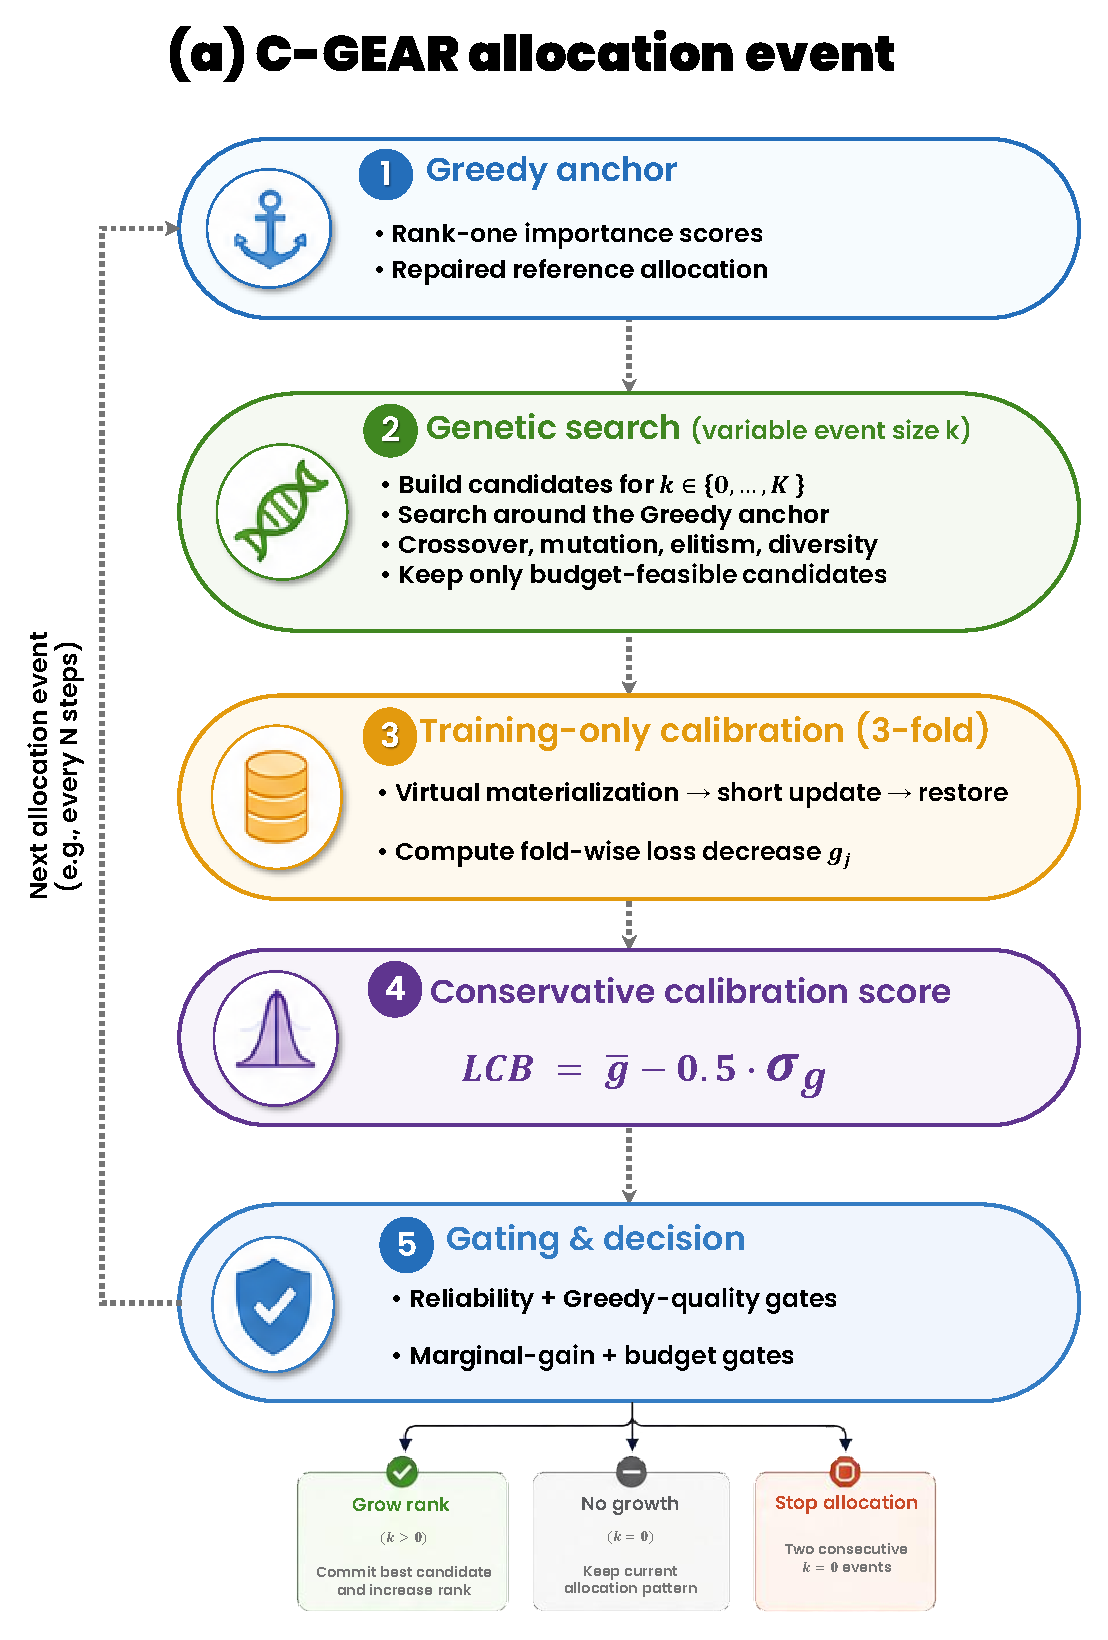
\includegraphics[width=\columnwidth]{../figures/cgear_allocation_event.pdf}
\caption{Overall C-GEAR allocation-event flow. Genetic search proposes feasible module sets; training-only calibration and conservative gates choose growth, no growth ($k=0$), or stopping after repeated no-growth events.}
\label{fig:method-overview}
\end{figure}

\begin{figure*}[!t]
\centering
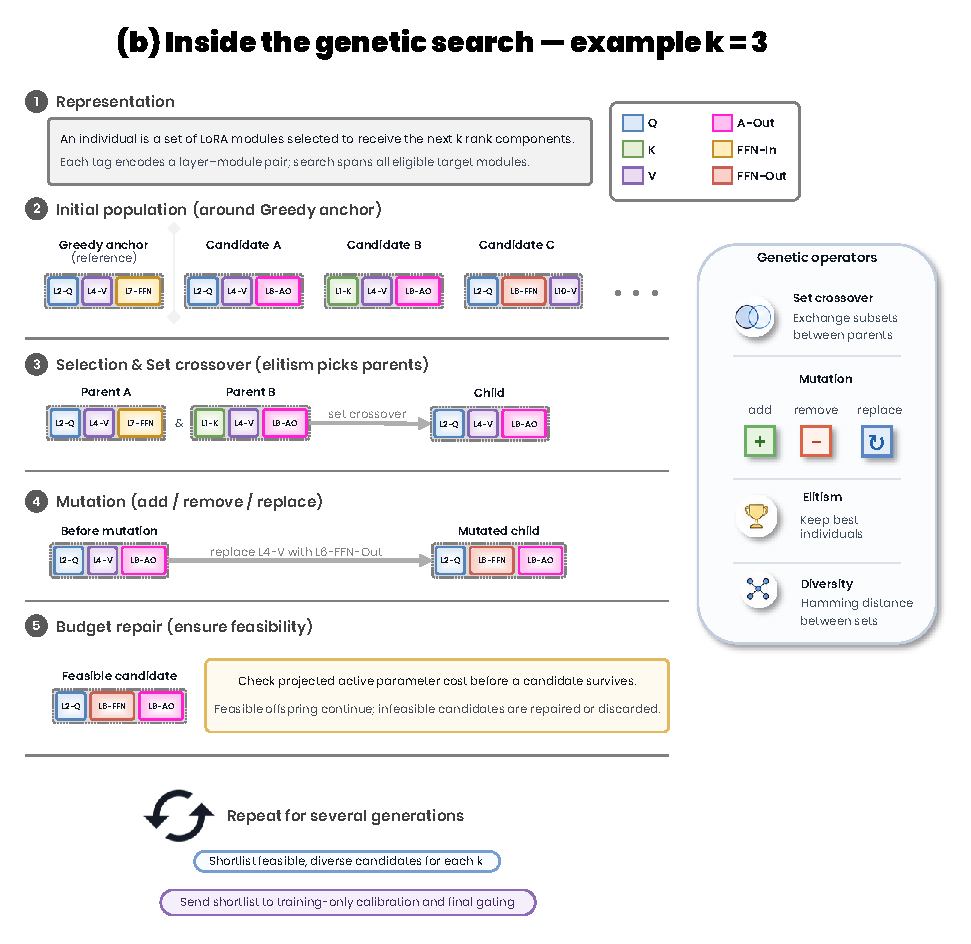
\includegraphics[width=0.88\textwidth]{../figures/cgear_genetic_search.pdf}
\caption{Inside the genetic search: an illustrative $k=3$ example, not a trace of a particular event. Individuals encode sets of layer--module pairs; Greedy anchoring, set crossover, add/remove/replace mutation, budget repair, elitism, and diversity produce a feasible calibration shortlist.}
\label{fig:genetic-search}
\end{figure*}

\section{Related Work}
Adaptive LoRA methods relax a single hand-chosen rank in different ways. AdaLoRA allocates a global budget by importance \cite{zhang2023adalora}; DyLoRA jointly trains a nested range of usable ranks \cite{valipour2023dylora}; SoRA learns sparse rank gates \cite{ding2023sora}; AutoLoRA uses meta-learning to tune layer ranks \cite{zhang2024autolora}; and dynamic-rank DoRA prunes rank-one components \cite{mao2024dora}. \mbox{IncreLoRA reverses pruning} by progressively adding components, avoiding a restrictive initial upper rank \cite{zhang2023increlora}. C-GEAR retains this incremental setting but targets a different gap: \emph{which combination} should grow at an event, by how much, and whether growth is warranted at all.

\section{Method / Proposed Approach}
Let module $i$ have active rank $r_i$ and dimensions $d_{\mathrm{in},i}$ and $d_{\mathrm{out},i}$. Its active adaptation cost is
\begin{equation}
C(\mathbf r)=\sum_i r_i(d_{\mathrm{in},i}+d_{\mathrm{out},i}), \qquad C(\mathbf r)\le B.
\end{equation}
At each event, C-GEAR first proposes budget-feasible allocations, then uses training-only evidence to decide among growth, no growth, and stopping (Figure~\ref{fig:method-overview}).

\subsection{Genetic Rank-Allocation Search}
An individual is the set of LoRA modules receiving the next $k$ rank-one components (Figure~\ref{fig:genetic-search}). Legal sizes are $k\in\{0,\ldots,K\}$, with the empty set representing a genuine no-growth action. The original IncreLoRA Greedy allocation remains the anchor and quality reference: C-GEAR retains a budget-repaired anchor and Greedy prefixes, enumerates nearby replacements, and seeds global populations with the anchor, cost/gain extremes, and random sets. Structural fitness combines normalized importance, complementary temporal interactions, redundancy, and relative parameter cost.

Tournament-selected parents undergo set crossover; mutation can add, remove, or replace modules. Deterministic repair substitutes cheaper modules or reduces cardinality until projected active cost satisfies $B$. Environmental selection retains a strong elite, then applies maximin normalized set-Hamming pressure, where membership-vector distance is $|A\mathbin{\triangle}B|/\max(|A|,|B|,1)$, to discourage population collapse. After the configured generations, representative feasible candidates form the shortlist. No post-hoc local search is used. Evolution therefore proposes allocations from training-derived signals; it does not optimize against RTE validation labels.

\subsection{Training-Only Calibration and Commit Decision}
Search alone cannot commit a change. Each shortlist candidate is virtually materialized, updated on three held-out \emph{training} folds, and restored with model, optimizer, rank, and random-number state unchanged. For loss decrease $g_j$ on fold $j$, the implemented conservative score is
\begin{equation}
S_{\mathrm{cal}}=\bar g-\lambda\sigma_g,\qquad \lambda=0.5.
\end{equation}
Here $\bar g$ rewards expected improvement, while $\sigma_g$ penalizes instability across folds. The score is a conservative LCB-style heuristic, not a formal 95\% confidence bound. A positive candidate must clear validity, marginal-gain, Greedy-quality, and budget gates; global-only candidates face a stricter improvement gate. Within the quality band, projected active cost is minimized before calibrated quality breaks ties. If none qualifies, $k=0$ preserves the pattern; two consecutive no-growth events stop allocation and begin ordinary consolidation training. Calibration uses training data only and never validation labels.

\section{Experimental Setup}
We perform a controlled local comparison on GLUE RTE \cite{wang2019glue} with \texttt{microsoft/deberta-v3-base} \cite{he2023debertav3}. Greedy IncreLoRA and C-GEAR use identical seeds 41--46, data order, model, targets, and optimization: 25 epochs (1,950 steps), sequence length 192, train/evaluation batches 32/8, AdamW at $1.2\!\times\!10^{-3}$, linear scheduling with 100 warm-up steps, weight decay 0.01, and FP16 on an RTX 4060 Laptop GPU. Allocation begins from rank one in 72 target modules and is considered every 100 steps. C-GEAR uses population 12, four generations, calibration top-6, budget ratio 0.94, and the fixed settings recorded by telemetry. RTE validation accuracy is the performance metric.

% Generated by regenerate_six_seed_analysis.py; do not edit by hand.
\begin{table}[!t]
\centering
\caption{Six-seed RTE results (mean $\pm$ sample SD). Accuracy and selected counts describe the same selected checkpoint; final counts are architectural.}
\label{tab:main-results}
\setlength{\tabcolsep}{3.6pt}
\begin{tabular}{lcc}
\toprule
Metric & Greedy IncreLoRA & C-GEAR \\
\midrule
Accuracy $\uparrow$ & 87.30 $\pm$ 0.84 & \textbf{88.09} $\pm$ 1.14 \\
Selected params $\downarrow$ & 828.0k $\pm$ 65.2k & \textbf{795.2k} $\pm$ 37.1k \\
Selected rank $\downarrow$ & 99.0 $\pm$ 27.8 & \textbf{86.7} $\pm$ 14.5 \\
Final params $\downarrow$ & 933.6k $\pm$ 5.3k & \textbf{804.1k} $\pm$ 39.3k \\
Final rank $\downarrow$ & 144.0 $\pm$ 0.0 & \textbf{89.7} $\pm$ 15.0 \\
\bottomrule
\end{tabular}
\end{table}


Efficiency is \emph{active model parameters}: the fixed task head plus components represented by the active rank pattern, not raw \texttt{requires\_grad} storage. ``Selected'' denotes the checkpoint chosen by validation accuracy after dynamic-rank restoration; ``final'' denotes the terminal allocation trajectory before that checkpoint is reloaded. We pair accuracy only with selected-checkpoint counts. This is a matched local reproduction, not a direct numerical comparison with differently configured results in the original IncreLoRA paper.

\section{Results \& Contributions}
\subsection{Outcome-Level Evidence}
Table~\ref{tab:main-results} gives the central comparison. C-GEAR raises mean accuracy by \AccuracyGain\ percentage points and wins/ties/loses \CgearWins/\CgearTies/\CgearLosses\ matched seeds. At those \emph{same selected checkpoints}, mean active parameters fall from 828,005 to 795,225 and mean active rank from 99.0 to 86.7. The primary paired reduction is \SelectedPairedReduction\%; the reduction computed from aggregate mean counts is 3.96\%, illustrating why the paired statistic must be labeled.

\begin{figure}[!t]
\centering
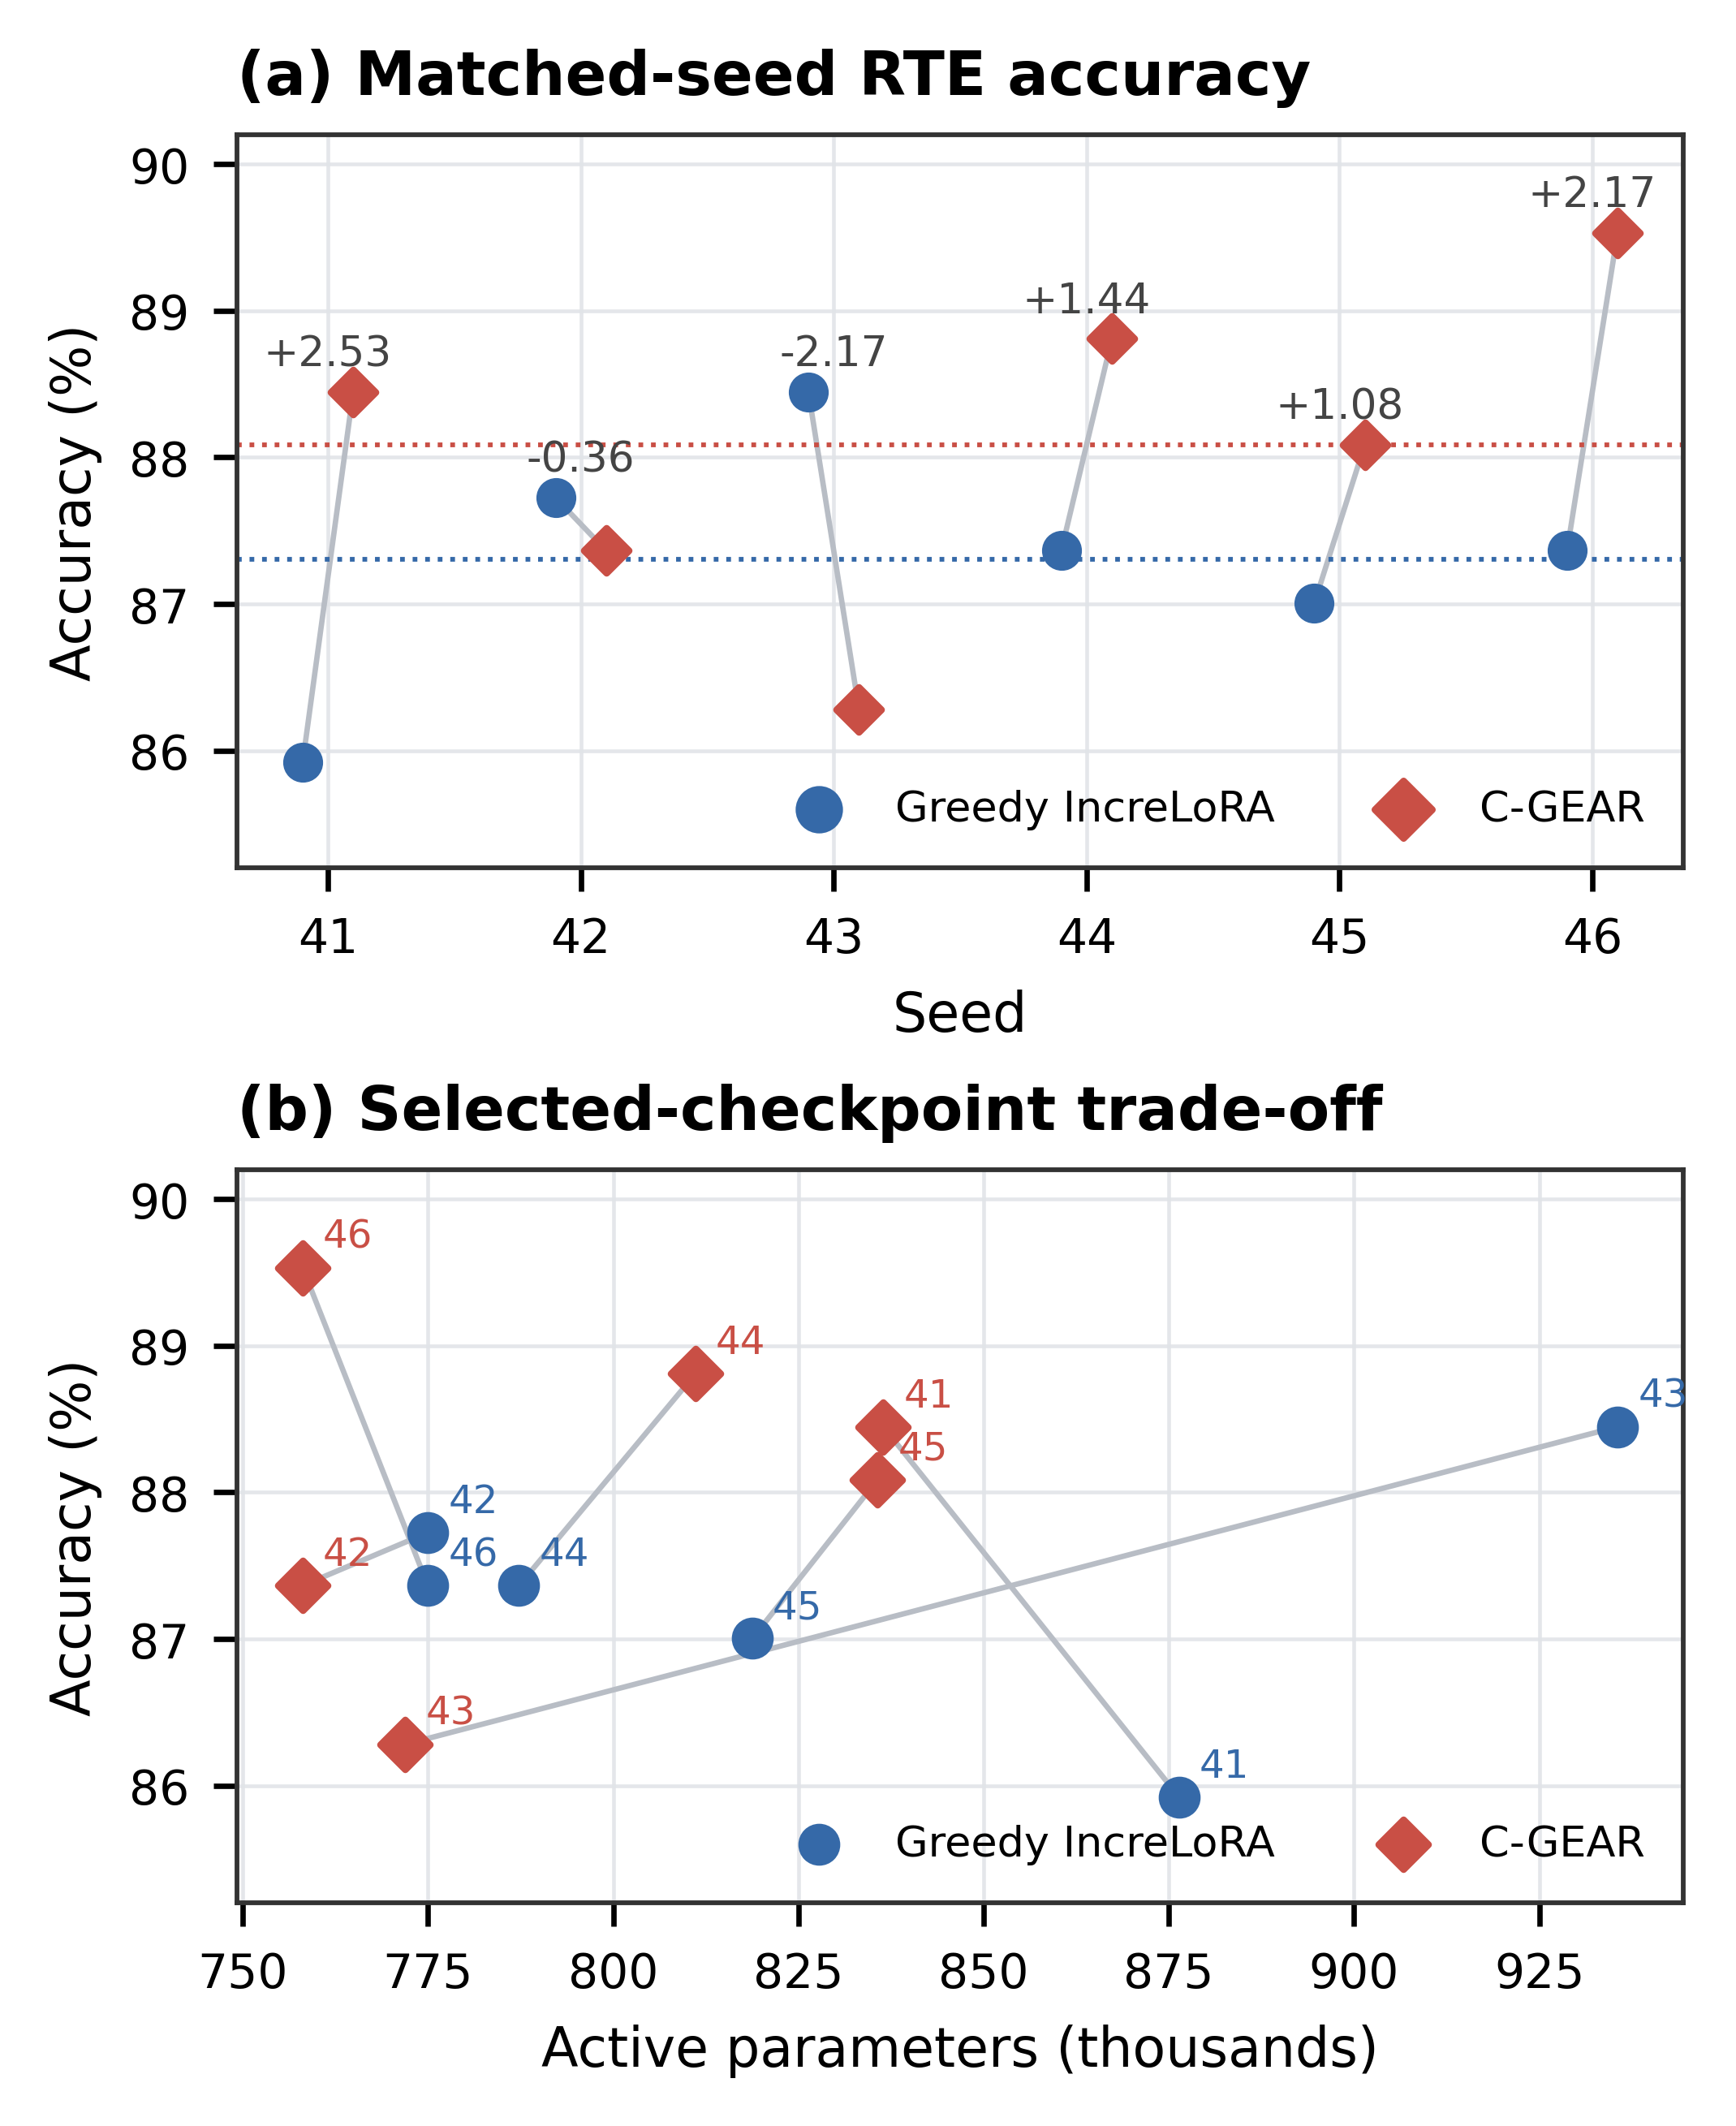
\includegraphics[width=\columnwidth]{../figures/accuracy_efficiency.png}
\caption{Matched results. (a) Per-seed accuracy and C-GEAR minus Greedy differences in percentage points. (b) Accuracy versus active parameters at the selected checkpoint; each gray segment joins a matched seed.}
\label{fig:tradeoff}
\end{figure}

Figure~\ref{fig:tradeoff} exposes rather than hides variation: C-GEAR loses on seeds 42 and 43, and selected efficiency is not lower for every pair. Nonetheless, the mean selected-checkpoint trade-off favors C-GEAR. Separately, final trajectories average 804,060 active parameters and rank 89.7, versus Greedy's 933,650 and rank 144; the mean paired final-parameter reduction is \FinalPairedReduction\%. These terminal counts do \emph{not} inherit selected-checkpoint accuracy.

\subsection{Mechanistic Analysis}
\begin{figure}[!t]
\centering
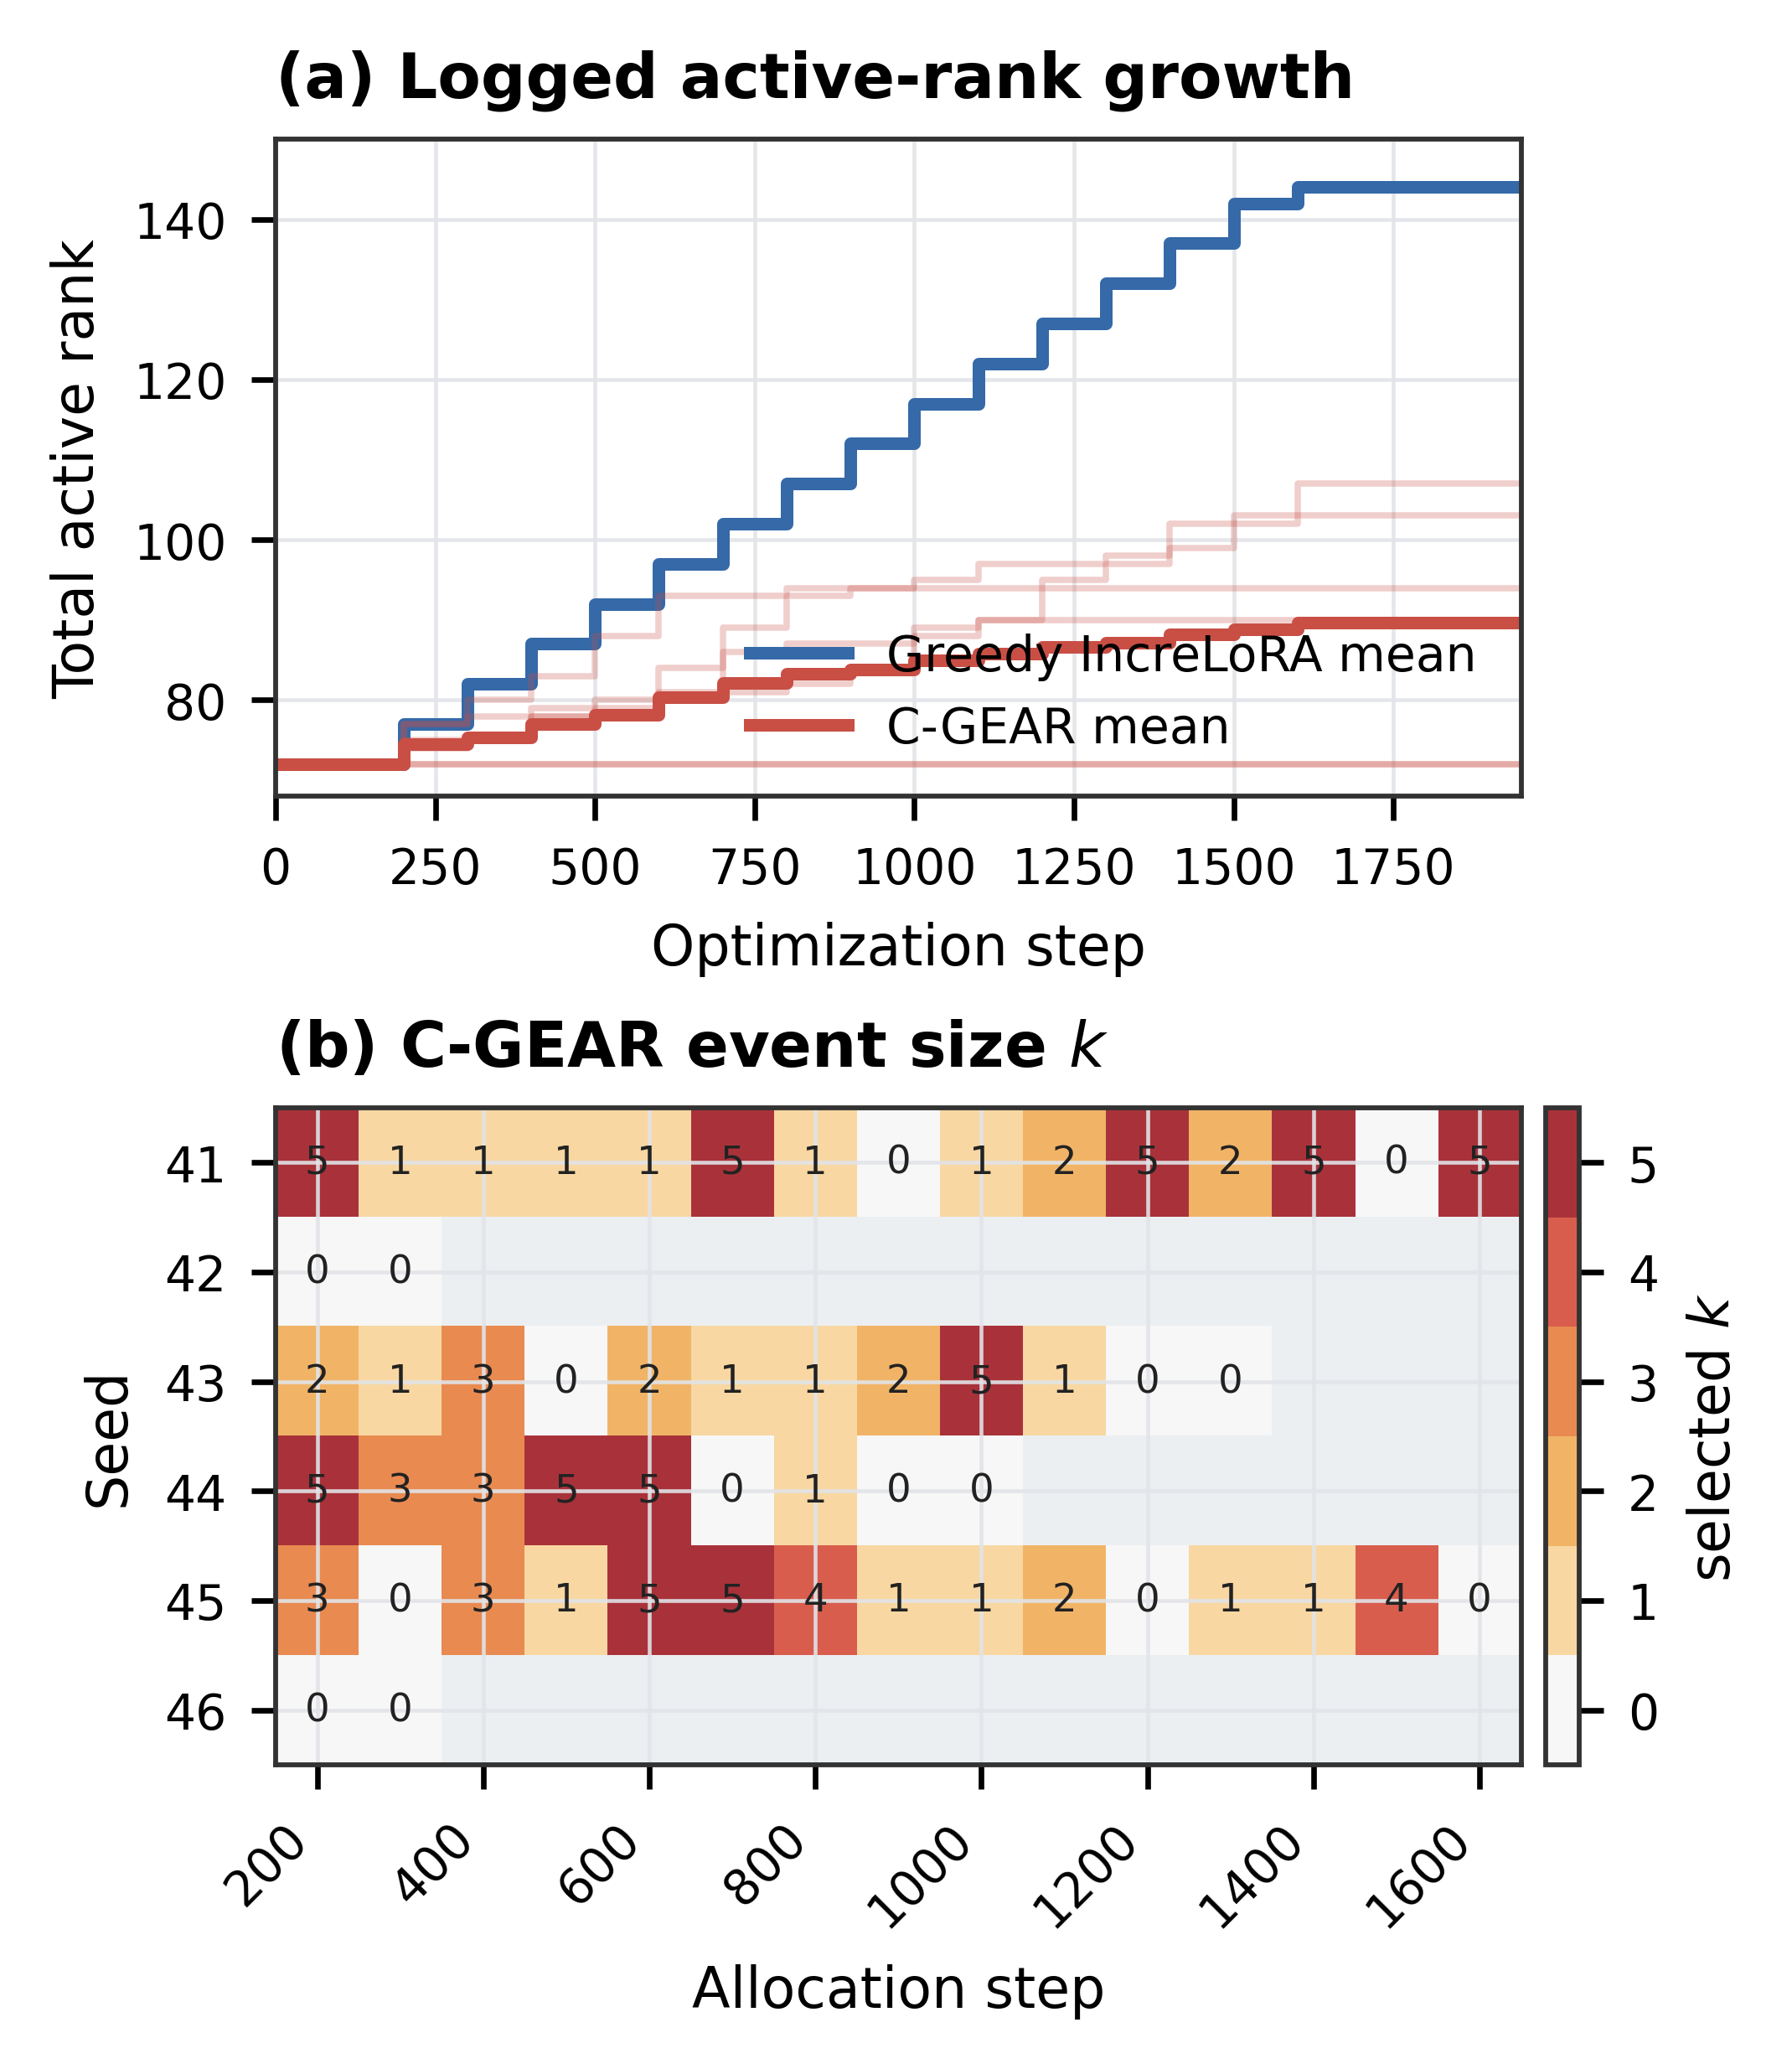
\includegraphics[width=\columnwidth]{../figures/rank_behavior.png}
\caption{Telemetry-derived growth. Top: all six trajectories and method means. Bottom: C-GEAR's selected event size; blank cells occur after allocation stops.}
\label{fig:growth}
\end{figure}

\begin{figure*}[!t]
\centering
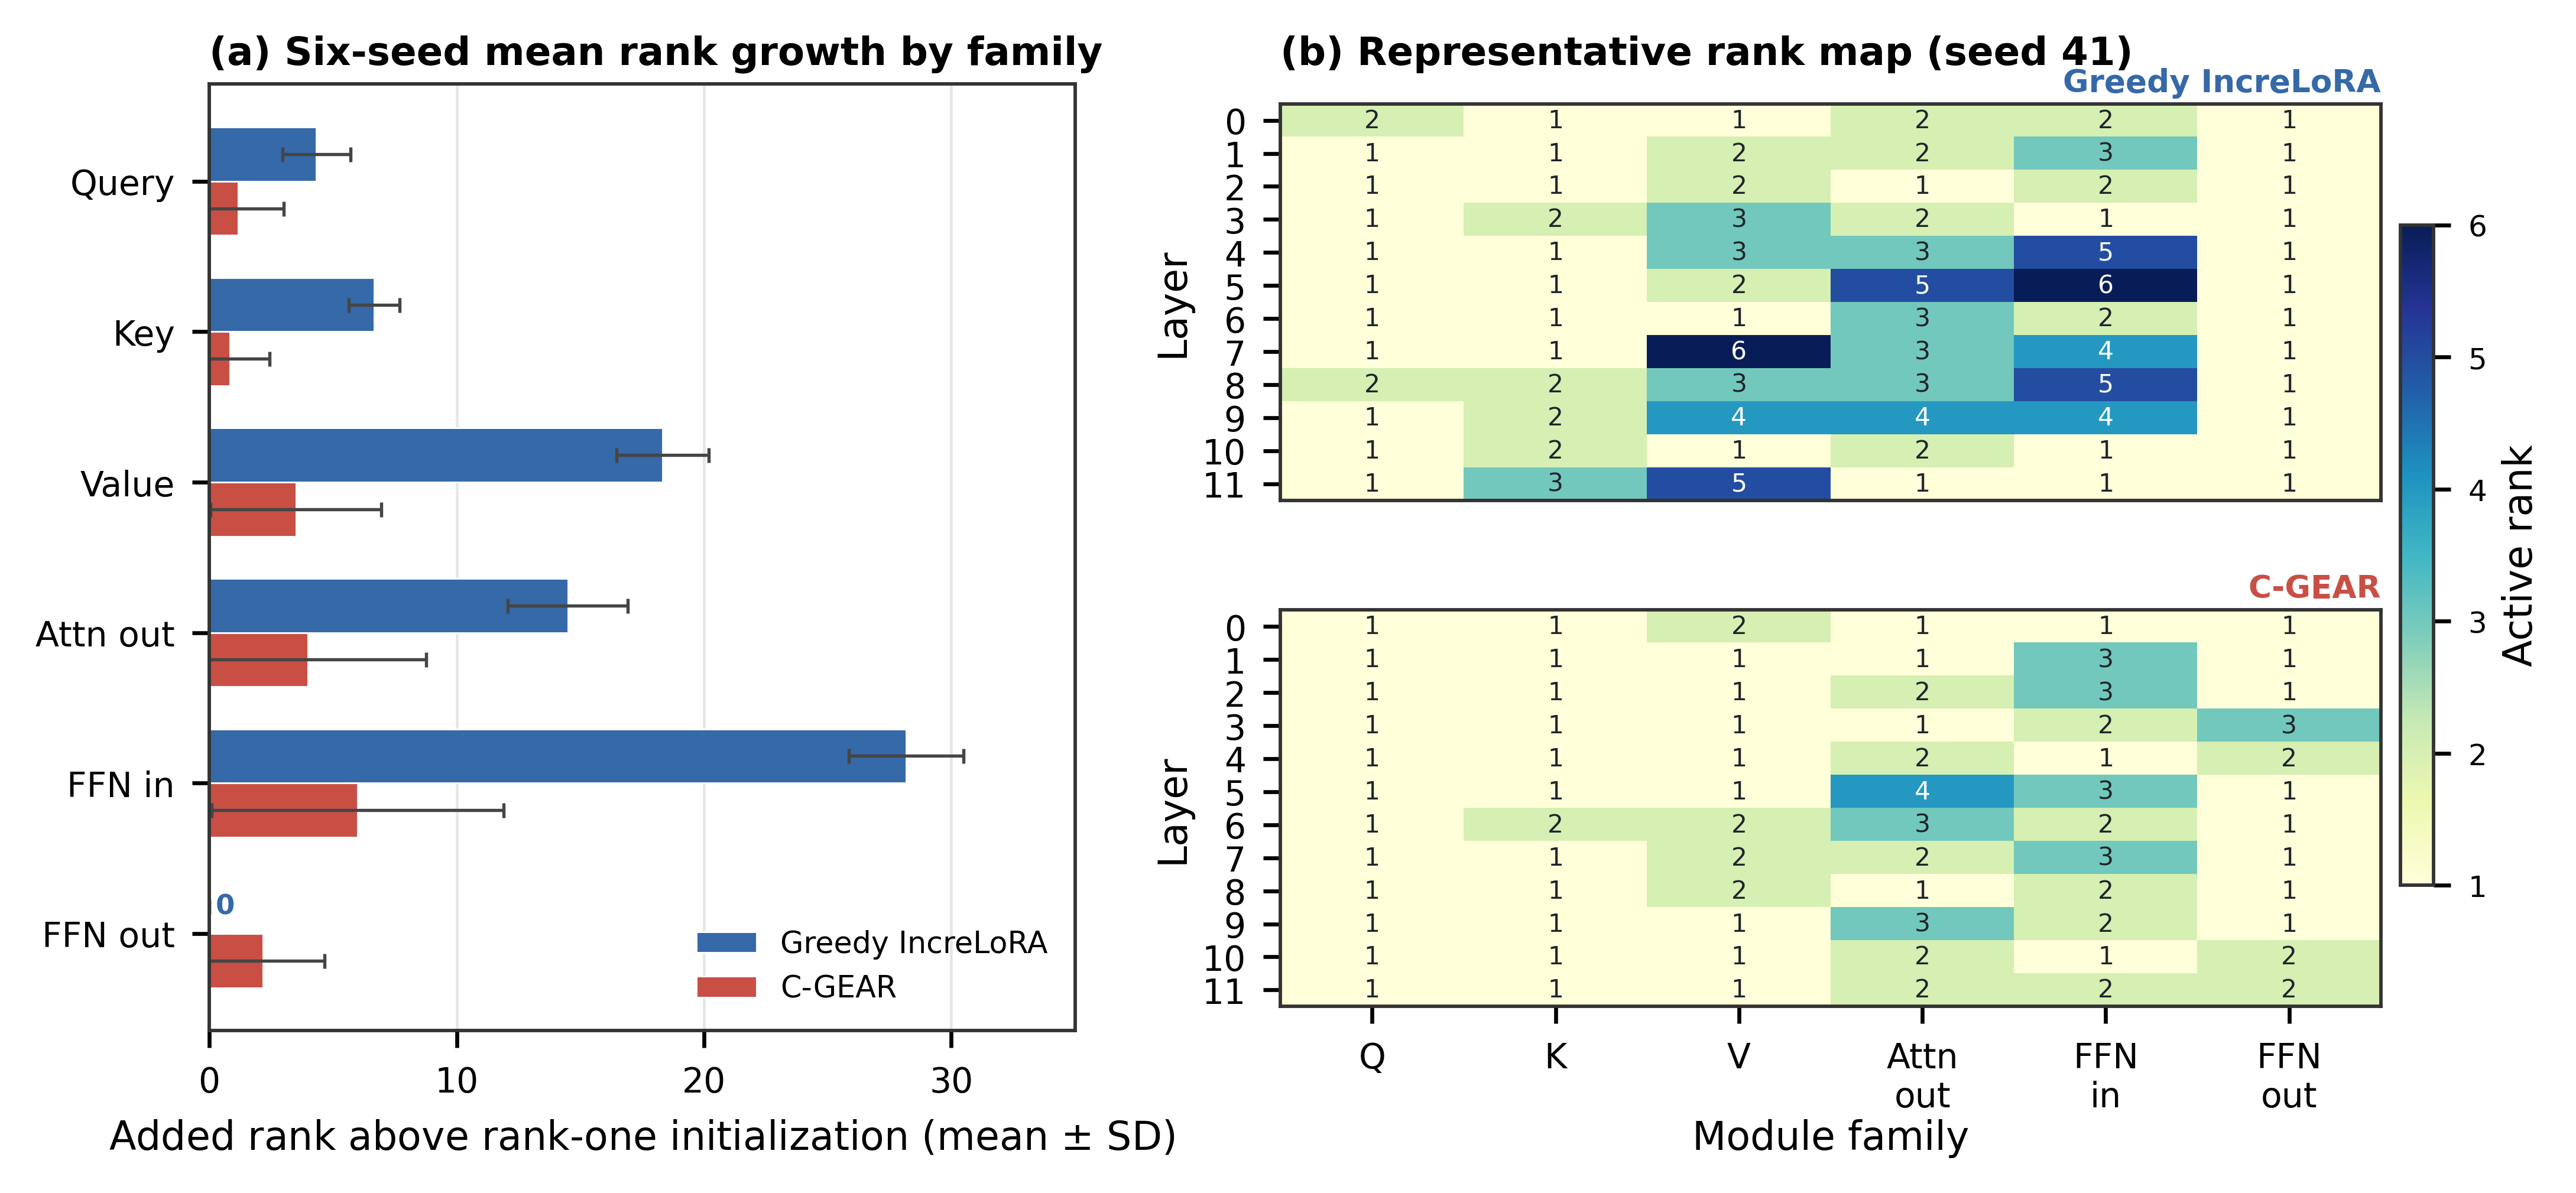
\includegraphics[width=0.99\textwidth]{../figures/mechanistic_rank_allocation.png}
\caption{Allocation structure. (a) Added rank above the common rank-one initialization, summed by family per seed and shown as mean $\pm$ sample SD over seeds 41--46. (b) Final layer $\times$ module-family maps for representative seed 41 under a shared active-rank scale. C-GEAR changes both the amount and placement of rank.}
\label{fig:allocation-structure}
\end{figure*}

Figure~\ref{fig:growth} separates rank-growth behavior from the outcome comparison. Greedy adds 72 ranks in every run and reaches rank 144. C-GEAR's 55 genuine calibrated decisions use every event size from $k=0$ to $k=5$: 15 select no growth, while the positive decisions produce seed-dependent terminal ranks from 72 to 107. Four runs stop after consecutive $k=0$ decisions; two instead enter the required final consolidation window. Optimization continues with the resulting fixed pattern after allocation stops.

Evolutionary exploration also affects committed allocations: global-GA candidates supply 13 of the 40 positive-growth decisions rather than every event reverting to the Greedy anchor. For representative seed 41, training-only calibration evaluates 105 shortlisted candidates over 15 events, selects global-GA candidates three times, and selects $k=0$ twice. Its full calibration history remains available as an auxiliary figure. Budget feasibility is enforced for every candidate; the representative seed-41 trace does not itself exhibit budget pressure.

Figure~\ref{fig:allocation-structure} shows that the smaller C-GEAR architectures are not proportional copies of Greedy. At seed 41, the final maps differ in 42 of 72 layer--family cells; C-GEAR assigns more rank in 12 cells despite using total rank 107 instead of 144. The four C-GEAR runs that grow beyond initialization develop non-uniform maps, whereas seeds 42 and 46 retain rank one throughout. Thus telemetry demonstrates changes in both \emph{how much} rank is allocated and, when growth occurs, \emph{where}; it does not establish that a particular pattern causally improves accuracy. Calibration and search add a measured 13.4\% mean wall-time overhead in this local setup.

\section{Future Work \& Conclusion}
The evidence is deliberately narrow: one GLUE task, one backbone, one laptop GPU, and six seeds. It does not establish statistical significance or cross-task generalization. Broader GLUE and model evaluation, larger seed sets, calibration/search ablations, and hardware-aware latency or memory objectives are natural next steps. Within this controlled study, C-GEAR supplies both a methodological improvement and a substantial implementation: it converts compulsory local Greedy growth into calibrated, budget-aware evolutionary decisions. Across six matched RTE seeds, it improves mean accuracy while using fewer selected-checkpoint parameters, and its final architectures grow substantially less.

\bibliographystyle{abbrv}
{\footnotesize\bibliography{references}}
\end{document}
